%*******************************************************************
% MAIN1
%*******************************************************************

\documentclass[a4paper,titlepage]{book}

%--------------------------------------------
% USEPACKAGES
%--------------------------------------------
\usepackage[utf8]{inputenc}
\usepackage[T1]{fontenc}
%!TEX encoding = UTF-8 Unicode
%\usefonttheme[onlymath]{serif}
\usepackage{listings}
\usepackage{lipsum}
\usepackage{caption}  
\usepackage[english]{babel}
\usepackage[swapnames]{frontespizio} 
\usepackage{textpos} %add the logo to the frametitle template using \addtobeamertemplate 
% https://texdoc.org/serve/textpos/0
\usepackage[hidelinks]{hyperref}
\urlstyle{same}
\usepackage{multicol}
\usepackage{graphics}
\usepackage{standalone}
\usepackage{multimedia}
\usepackage{media9}
\usepackage{graphicx}
\usepackage{empheq}
\usepackage{color}
\usepackage{siunitx}
\usepackage[many]{tcolorbox}
\usepackage{verbatim}
\usepackage{subfigure}
\usepackage{listings}
\usepackage{xcolor}
%\usepackage{palatino}
%\usepackage{euler}

%----------------------------
% ABSTRACT
%---------------------------
\usepackage{fancyhdr}


\begin{document}

%--------------------------------------------
% FRONTESPIZION
%--------------------------------------------
%https://tex.stackexchange.com/questions/161179/package-frontespizio
%https://ctan.mirror.garr.it/mirrors/ctan/macros/latex/contrib/frontespizio/frontespizio.pdf
% TO COMPILE:
% pdflatex [file].tex
% pdflatex [file-frn].tex
% pdflatex [file].tex
\begin{frontespizio}
    \begin{Preambolo*}
        %\usepackage{times}
        \usepackage{palatino}
        \newcommand{\VOF}{\textsc{vof}}
    \end{Preambolo*}
    \Istituzione{University of Pisa}
    \Logo[6.0cm]{figures/logo_unipi.jpg} 
    \Divisione{Department of Natural, Mathematical and Physical Sciences} 
    \Scuola{Master’s degree in Physics}
    \Titolo{Triggers fragmentation studies for FOOT experiment}
    \Relatore{Luca Galli} 
    \NRelatore{Thesis advisor}{} 
    \Correlatore{Bisogni Maria Giuseppina}
    \NCorrelatore{Research supervisor}{Research supervisors} 
    \NCandidato{Candidate}
    \Candidato{Lorenzo Marini} 
    \Piede{Academic Year 2021–2022}
\end{frontespizio}

% pdflatex [file].tex
% pdflatex [file-frn].tex
% pdflatex [file].tex

    %--------------------------------------------
    % DEDICA
    %--------------------------------------------
    %\begin{flushright}
Dedicato a qualcuno...
\end{flushright}

    %--------------------------------------------
    % ABSTRACT
    %--------------------------------------------    
    \newenvironment{abstract}%
    {\cleardoublepage\thispagestyle{empty}\null\vfill\begin{center}%
    \bfseries\abstractname\end{center}}%
    {\vfill\null}
        \begin{abstract}
        This is the abstract.
        \end{abstract}




    %--------------------------------------------
    % INDICI
    %--------------------------------------------
    \tableofcontents
    \listoffigures
    \listoftables

    %--------------------------------------------
    % CAP 1 - CHARGE PARTICLE THERAPHY
    %--------------------------------------------
    \chapter{Charge Particle Therapy}

\lipsum[1-3]

\begin{equation}
    F = ma
\end{equation}



\begin{figure}
    \centering    
        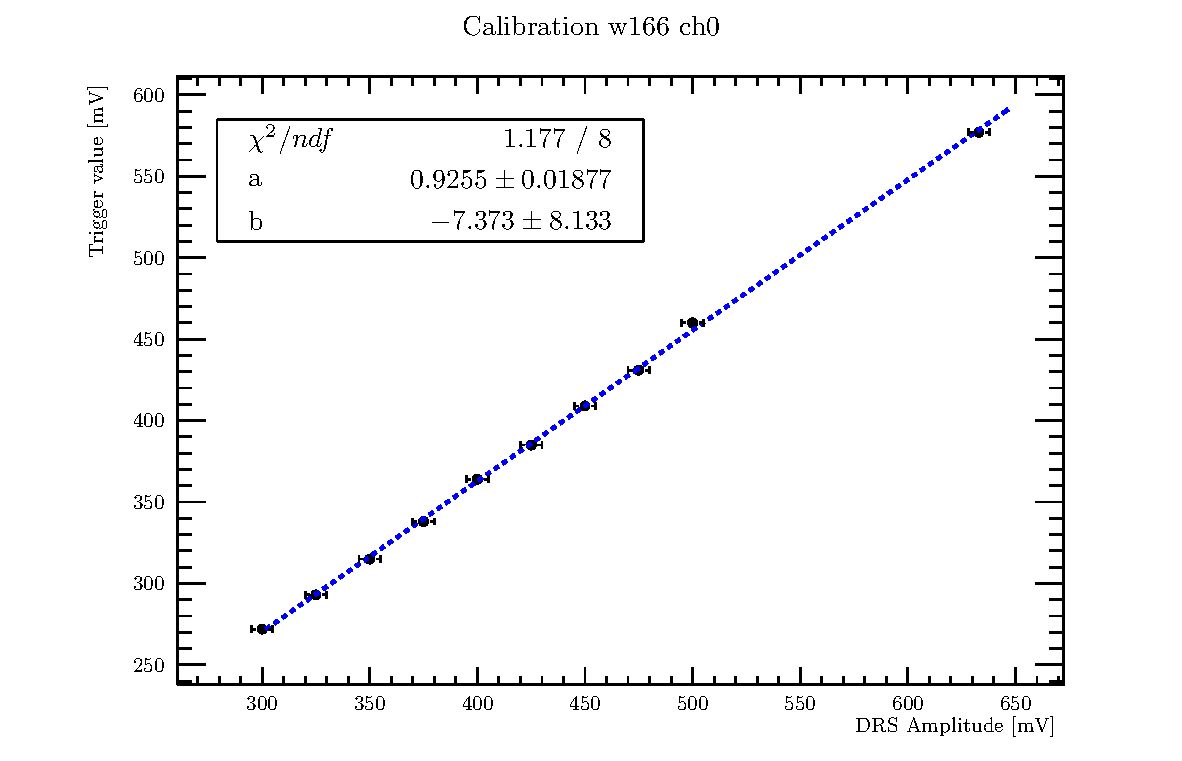
\includegraphics[width=10cm]{figures/ch0.pdf}
        \caption{$y=x$}
        \label{fig:y equals x}
\end{figure}








        \section{Prima sezione}


Qui ci scrivo qualcosa.
            \subsection{Electron magnetic energy loss of heavy charged particles}

\lipsum[1-3]\cite{Pan}.
            \subsection{Multiple Coulomb Scattering}

Scrivo qualcosa\cite{Pan}.
            \subsection{Nuclear interaction}

Scrivo qualcosa\cite{Pan}.
            \subsection{Range}

Scrivo qualcosa\cite{Pan}.
        \section{Radiobiology in CPT}


Qui ci scrivo qualcosa.
            \subsection{Dose deposition}

\lipsum[1-3]\cite{Pan}.
            \subsection{DNA damage}

Scrivo qualcosa\cite{Pan}.
            \subsection{Linear Energy Transfer}

Scrivo qualcosa\cite{Pan}.
            \subsection{Cells survival models}

\lipsum[1-3]
            \subsection{Relative Biological Effectiveness}

Scrivo qualcosa\cite{Pan}.
        \section{Thesis objectives}

\lipsum[1-3]


    %--------------------------------------------
    % CAP 2 - THE FOOT EXPERIMENT
    %--------------------------------------------
    \chapter{The FOOT experiment}


Prova del capitolo 1.

\begin{equation}
    F = ma
\end{equation}


\begin{equation}
    F = ma
\end{equation}


\begin{equation}
    F = ma
\end{equation}


\begin{equation}
    F = ma
\end{equation}

\begin{figure}
    \centering
    \begin{subfigure}[b]{0.15\textwidth}
        \centering
        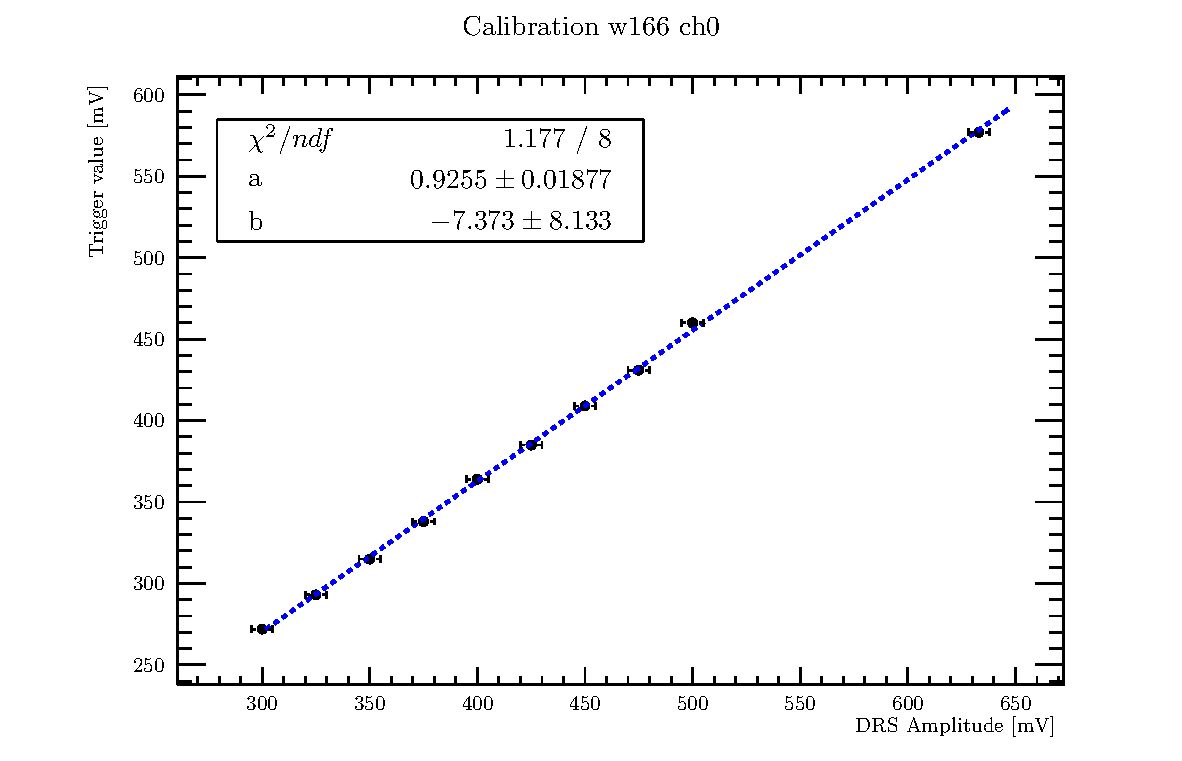
\includegraphics[width=2cm]{figures/ch0.pdf}
        \caption{$y=x$}
        \label{fig:y equals x}
    \end{subfigure}
    \hfill
    \begin{subfigure}[b]{0.15\textwidth}
        \centering
        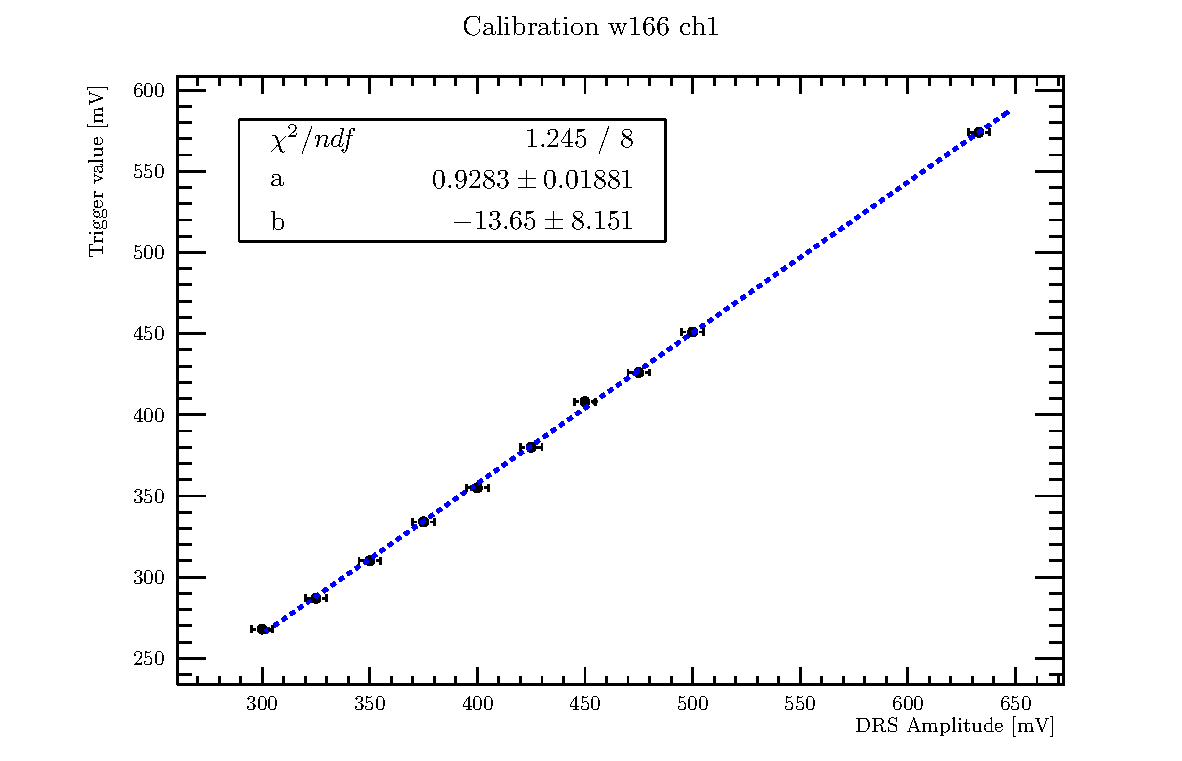
\includegraphics[width=2cm]{figures/ch1.pdf}
        \caption{$y=3sinx$}
        \label{fig:three sin x}
    \end{subfigure}
\end{figure}







        \section{Prima sezione}


Qui ci scrivo qualcosa.
        \section{Experimentla setup}


\lipsum[1-3]
            \subsection{Upstream region}

Scrivo qualcosa\cite{Pan}.
            \subsection{Tracking system}

Scrivo qualcosa\cite{Pan}.
            \subsection{Downstream region}

\lipsum[1-3]\cite{Pan}.
        \section{Prima sezione}


Qui ci scrivo qualcosa.

    %--------------------------------------------
    % CAP 3 - MATERIALS AND METHODS
    %--------------------------------------------
    \chapter{Capitolo 1}


Prova del capitolo 1.

\begin{equation}
    F = ma
\end{equation}


\begin{equation}
    F = ma
\end{equation}


\begin{equation}
    F = ma
\end{equation}


\begin{equation}
    F = ma
\end{equation}



\begin{figure}
    \centering
    \begin{subfigure}[b]{0.15\textwidth}
        \centering
        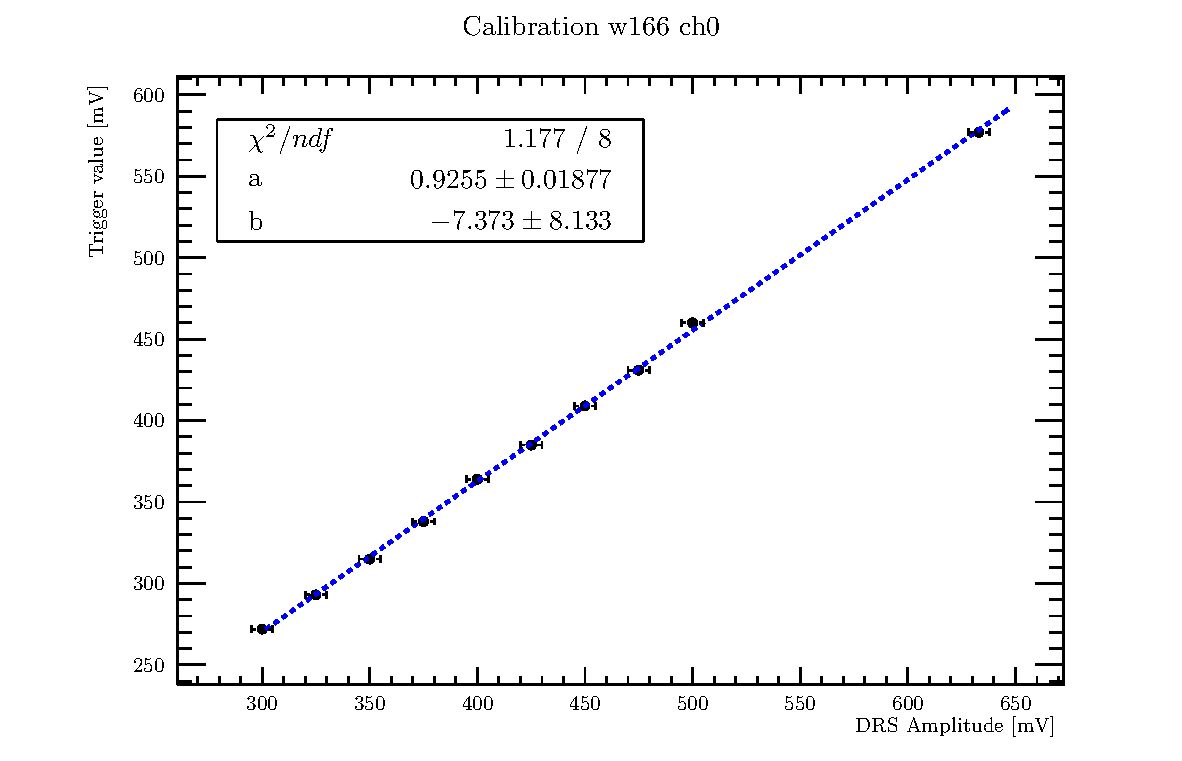
\includegraphics[width=\textwidth]{figures/ch0.pdf}
        \caption{$y=x$}
        \label{fig:y equals x}
    \end{subfigure}
    \hfill
    \begin{subfigure}[b]{0.15\textwidth}
        \centering
        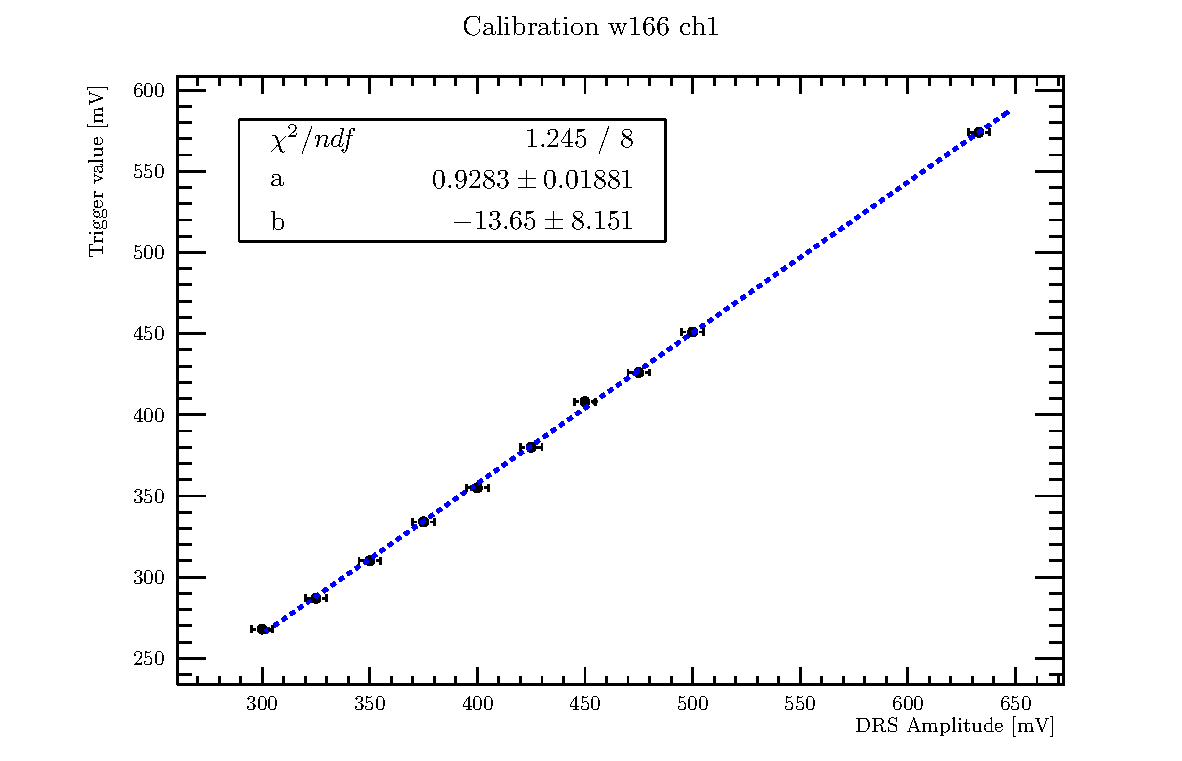
\includegraphics[width=\textwidth]{figures/ch1.pdf}
        \caption{$y=3sinx$}
        \label{fig:three sin x}
    \end{subfigure}
\end{figure}








        \section{Prima sezione}


Qui ci scrivo qualcosa.
        \section{Detection system}

\lipsum[1-3]
            \subsection{Sottosezione}

Scrivo qualcosa\cite{Pan}.
            \subsection{Sottosezione}

Scrivo qualcosa\cite{Pan}.
            \subsection{The WaveDAQ system}

Scrivo qualcosa\cite{Pan}.
        \section{Trigger update}


Qui ci scrivo qualcosa.
        \subsection{WaveDREAM channels calibration}

\lipsum[1-3]\cite{Pan}.
        \section{Data taking}


\lipsum[1-3]
            \input{cap3/3_3_3_cnao_setup.tex}
        \section{Prima sezione}


Qui ci scrivo qualcosa.
            \subsection{Start Counter waveforms analysis}

Scrivo qualcosa\cite{Pan}.
            \subsection{TOF-Wall waveforms analysis}

Scrivo qualcosa\cite{Pan}.
            \subsection{Clock analysis}

\lipsum[1-3]\cite{Pan}.
            \subsection{Time resolution}

Scrivo qualcosa\cite{Pan}.
            \subsection{Time of flight evaluation}

Scrivo qualcosa\cite{Pan}.
            \subsection{Charge evaluation}

\lipsum[1-3]\cite{Pan}.
            \subsection{Sottosezione}

Scrivo qualcosa\cite{Pan}.

    %--------------------------------------------
    % CAP 4 - RESULT AND DISCUSSION
    %--------------------------------------------
    \chapter{Capitolo 1}


Prova del capitolo 1.

\begin{equation}
    F = ma
\end{equation}


\begin{equation}
    F = ma
\end{equation}


\begin{equation}
    F = ma
\end{equation}


\begin{equation}
    F = ma
\end{equation}



\begin{figure}
    \centering
    \begin{subfigure}[b]{0.15\textwidth}
        \centering
        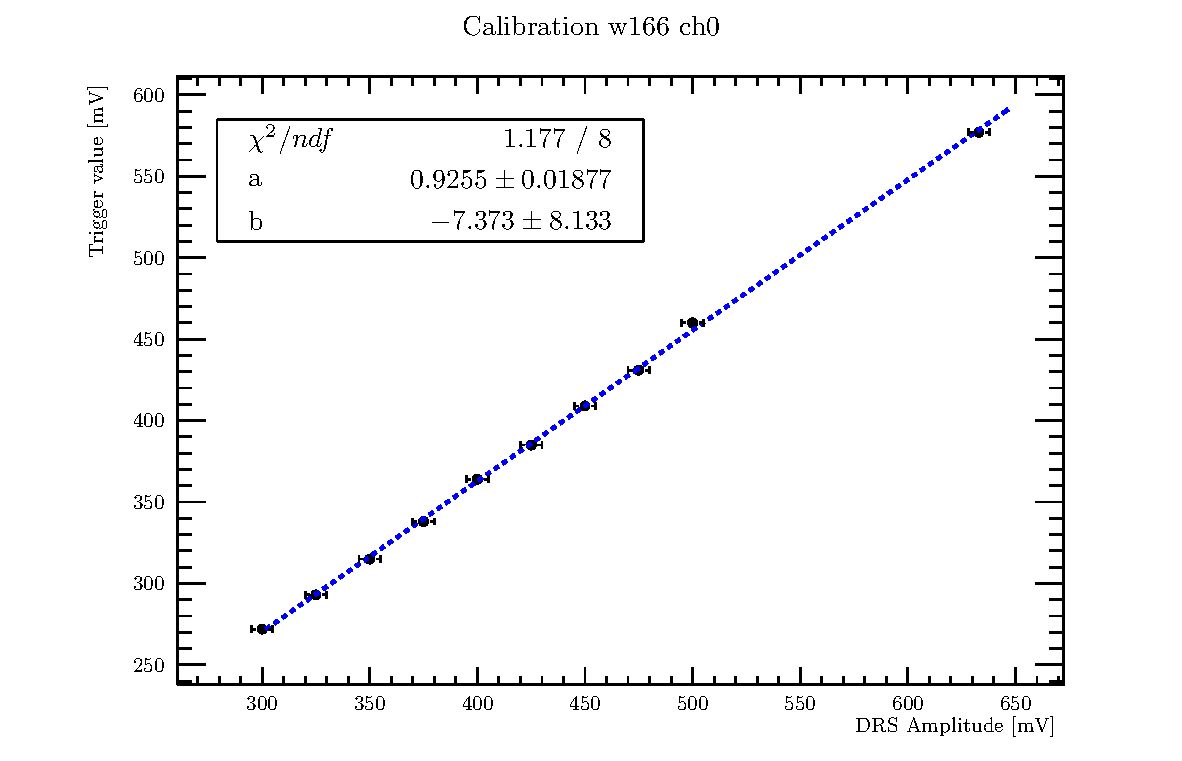
\includegraphics[width=\textwidth]{figures/ch0.pdf}
        \caption{$y=x$}
        \label{fig:y equals x}
    \end{subfigure}
    \hfill
    \begin{subfigure}[b]{0.15\textwidth}
        \centering
        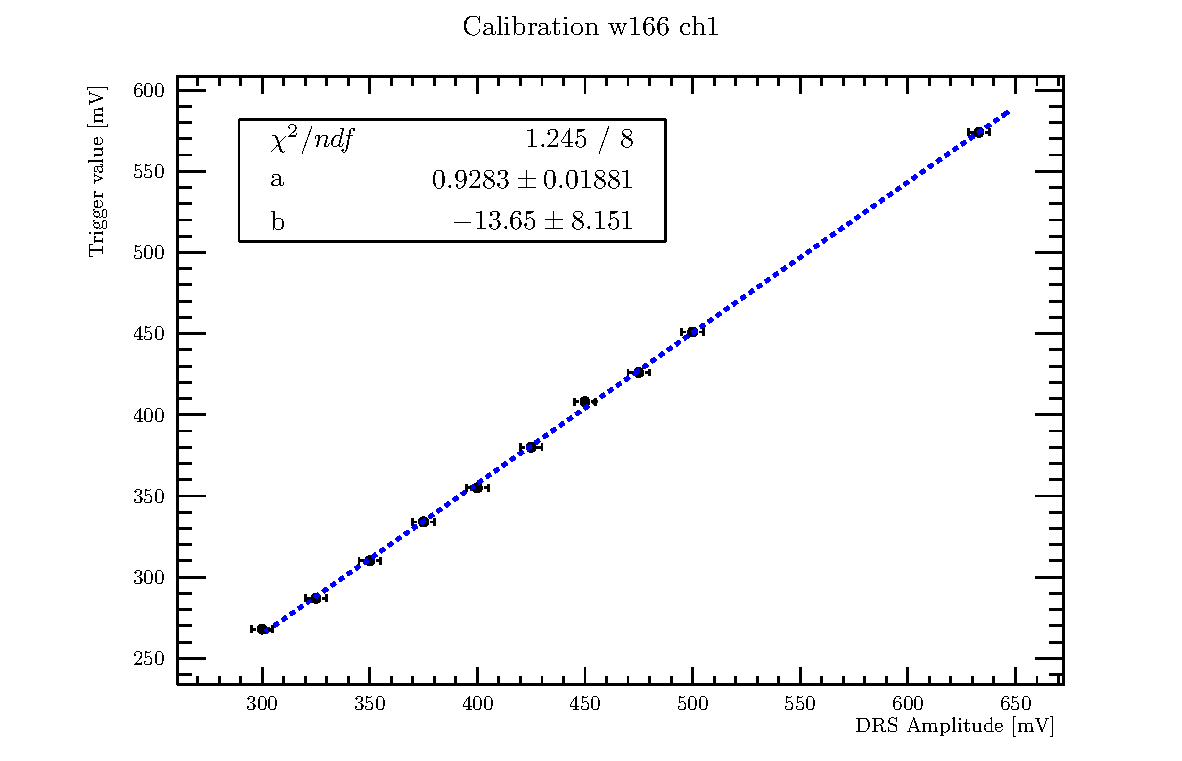
\includegraphics[width=\textwidth]{figures/ch1.pdf}
        \caption{$y=3sinx$}
        \label{fig:three sin x}
    \end{subfigure}
\end{figure}








        \section{Trigger efficency}


Qui ci scrivo qualcosa.
        \section{Charge reconstruction}


Qui ci scrivo qualcosa.

    %--------------------------------------------
    % APPENDIX
    %--------------------------------------------
    \appendix
    \chapter{Capitolo 1}


Prova del capitolo 1.

\begin{equation}
    F = ma
\end{equation}


\begin{equation}
    F = ma
\end{equation}


\begin{equation}
    F = ma
\end{equation}


\begin{equation}
    F = ma
\end{equation}



\begin{figure}
    \centering
    \begin{subfigure}[b]{0.15\textwidth}
        \centering
        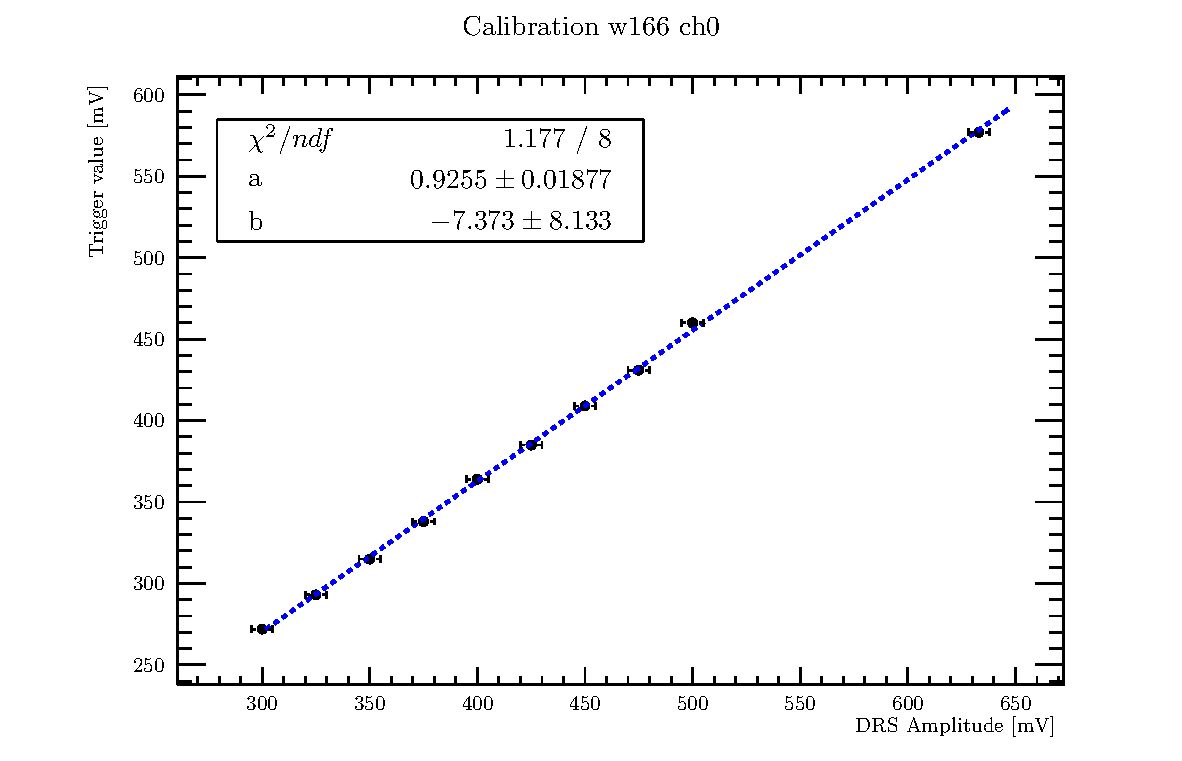
\includegraphics[width=\textwidth]{figures/ch0.pdf}
        \caption{$y=x$}
        \label{fig:y equals x}
    \end{subfigure}
    \hfill
    \begin{subfigure}[b]{0.15\textwidth}
        \centering
        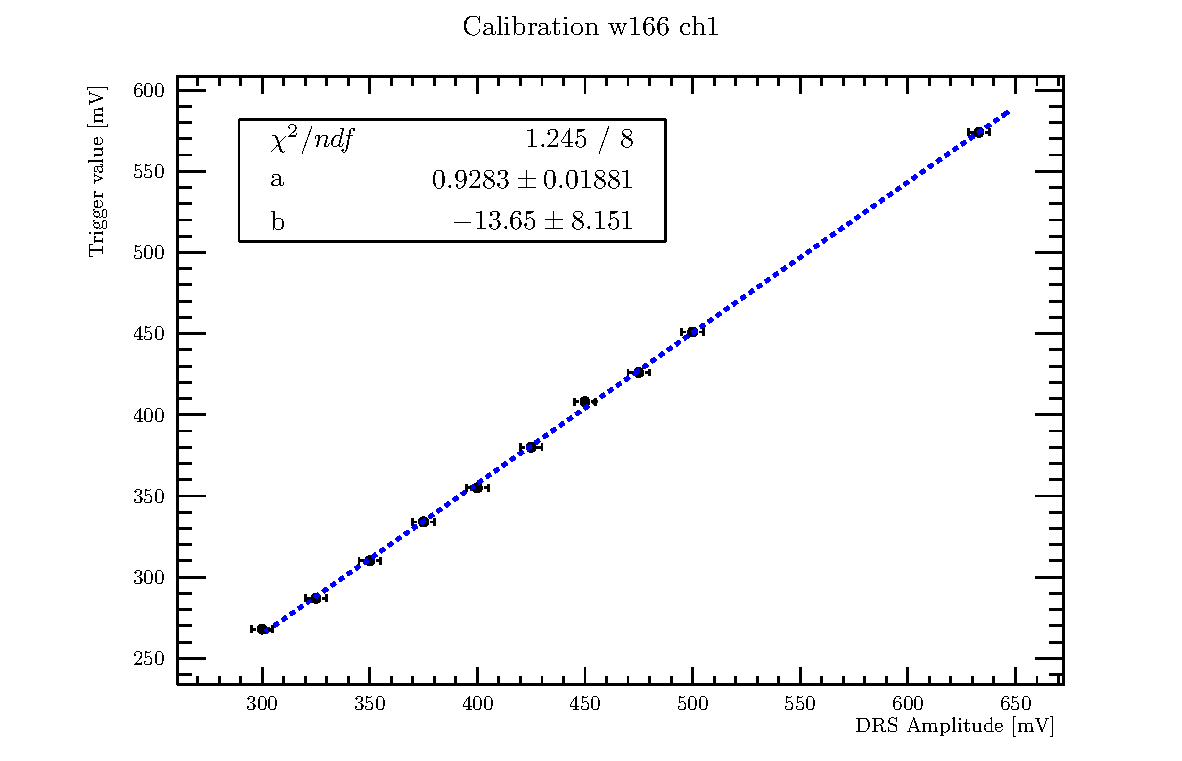
\includegraphics[width=\textwidth]{figures/ch1.pdf}
        \caption{$y=3sinx$}
        \label{fig:three sin x}
    \end{subfigure}
\end{figure}








    
    %--------------------------------------------
    % BIBLIOGRAPHY
    %--------------------------------------------
    \bibliographystyle{alpha}
    \bibliography{biblio}
    % pdflatex [filename].tex
    % bibtex [filename]
    % pdflatex [filename].tex
    % pdflatex [filename].tex
    % https://tex.stackexchange.com/questions/450863/using-bibtex-with-pdflatex

    %--------------------------------------------
    % ACKONWLEDGEMENTS
    %--------------------------------------------
    \chapter*{Acknowledgements}
I want to thank...
%--------------------------------------------
% END
%--------------------------------------------
\end{document}
